\chapter{Consumo energetico}
\label{chap:consumi}

Questo capitolo stima il consumo energetico dei sensori e del nodo che li ospita. L'analisi è a titolo informativo e usa i valori dichiarati dai produttori, perché non si dispone di strumentazione di misura (né multimetro né resistenze di shunt), come concordato con il relatore.

Il capitolo è organizzato come segue. La Sezione~\ref{sec:consumi-dati} riprende i consumi dei sensori dal Capitolo~\ref{chap:moduli} e vi aggiunge quelli del microcontrollore. La Sezione~\ref{sec:consumi-nodi} li somma nelle configurazioni del nodo usate nella tesi e in quelle a cui può aspirare il nodo del progetto, e la Sezione~\ref{sec:autonomia} ne ricava l'autonomia a batteria. La Sezione~\ref{sec:architettura-ibrida} mostra l'architettura ibrida PIR + mmWave che ne discende per DIPME.

\section{Dati di partenza}
\label{sec:consumi-dati}

Le correnti dei sensori sono già nelle specifiche del Capitolo~\ref{chap:moduli}
(Tabella~\ref{tab:c3-1} per l'\ldb, Sezione~\ref{sec:c3-2} per l'\ldc,
Tabella~\ref{tab:c3-12} per il PIR). Qui si riprendono soltanto i valori che entrano nei
conti. L'\ldb\ assorbe in media 80~mA a 5~V, pari a circa 400~mW, mentre l'\ldc\
assorbe 50~mA a 3,3~V, circa 165~mW. L'\pir\ assorbe meno di 50~\textmu A, cioè circa
0,3~mW. Il rapporto fra i due estremi è il dato strutturale di tutto il capitolo,
perché il radar consuma circa 1600 volte la corrente del PIR.

Il dimostratore del progetto monta un microcontrollore STM32WLE con radio LoRa e un PIR digitale Panasonic EKMB139~\cite{callisto2026dipme}, componenti della classe a bassissimo consumo per i nodi a batteria, diversi da quelli del kit. I valori di questo capitolo si riferiscono al kit usato negli esperimenti, ma la conclusione sull'ordine di grandezza del divario non dipende da quale PIR o microcontrollore si consideri.

Il microcontrollore è il componente che manca al Capitolo~\ref{chap:moduli}. La
Tabella~\ref{tab:consumi-esp32} riporta le correnti dell'ESP32-WROOM-32 per modalità
operativa, dal datasheet Espressif~\cite{esp32datasheet}.

\begin{table}[htbp]
\centering
\caption{Consumo dell'ESP32-WROOM-32 per modalità operativa, dal datasheet
Espressif~\cite{esp32datasheet}.}
\label{tab:consumi-esp32}
\small
\begin{tabular}{@{}lr@{}}
\toprule
\textbf{Modalità} & \textbf{Corrente} \\
\midrule
Attivo, WiFi in trasmissione (picco) & 160--260~mA \\
Attivo, WiFi connesso in ascolto & 95--100~mA \\
Modem-sleep (CPU attiva a 80--240~MHz, WiFi spento) & 20--68~mA \\
Light-sleep & 0,8~mA \\
Deep-sleep (solo dominio RTC) & 0,01~mA \\
\bottomrule
\end{tabular}
\end{table}

\section{Il nodo completo}
\label{sec:consumi-nodi}

Sommando microcontrollore e sensore si ottengono le configurazioni usate in questa
tesi e quelle rilevanti per il progetto (Tabella~\ref{tab:consumi-nodi}). Le prime tre sono le configurazioni usate nella tesi, le ultime due quelle a cui può aspirare il nodo del progetto.

\begin{table}[htbp]
\centering
\caption{Consumo stimato del nodo completo nelle configurazioni di interesse, somma
dei valori di datasheet.}
\label{tab:consumi-nodi}
\small
\begin{tabular}{@{}lrr@{}}
\toprule
\textbf{Configurazione} & \textbf{Corrente} & \textbf{Potenza a 5~V} \\
\midrule
ESP32 attivo + \ldb\ + WiFi (web UI) & 180--260~mA & 0,9--1,3~W \\
ESP32 attivo + \ldb\ (logger seriale) & 110--150~mA & 0,55--0,75~W \\
ESP32 attivo + \ldc & 80--120~mA & 0,4--0,6~W \\
ESP32 attivo + PIR & 30--70~mA & 0,15--0,35~W \\
ESP32 in deep-sleep + PIR, sveglia su interrupt & $\mathbf{0{,}06}$~\textbf{mA} & 0,3~mW \\
\bottomrule
\end{tabular}
\end{table}

L'ultima riga è il punto chiave, perché l'uscita digitale del PIR può risvegliare
l'ESP32 dal deep-sleep con un interrupt su GPIO. Il nodo può quindi restare in attesa a
costo praticamente nullo, con il PIR nel ruolo di guardiano.

\section{Autonomia a batteria}
\label{sec:autonomia}

Con una cella litio-ione 18650 da 3000~mAh e un rendimento del regolatore dell'85\,\%
si ottengono le autonomie di Tabella~\ref{tab:autonomia}. La Figura~\ref{fig:consumi} le riassume
insieme ai consumi dei componenti.

\begin{table}[htbp]
\centering
\caption{Autonomia stimata, calcolata come capacità per rendimento diviso la corrente assorbita, trascurando la differenza fra la tensione della cella e quella dei moduli. Nel regime dormiente il fattore limitante è l'autoscarica della cella, non il consumo.}
\label{tab:autonomia}
\small
\begin{tabular}{@{}lrr@{}}
\toprule
\textbf{Scenario} & \textbf{Corrente media} & \textbf{Autonomia} \\
\midrule
Nodo mmWave attivo con WiFi (\ldb) & 200~mA & 13~h \\
Nodo mmWave attivo senza WiFi continuo & 130~mA & 20~h \\
Nodo PIR sempre attivo (ESP32 in modem-sleep) & 25~mA & 4 giorni \\
Nodo dormiente (deep-sleep, PIR come guardiano) & 0,06~mA & 4,9 anni al solo consumo \\
\bottomrule
\end{tabular}
\end{table}

\begin{figure}[htbp]
\centering
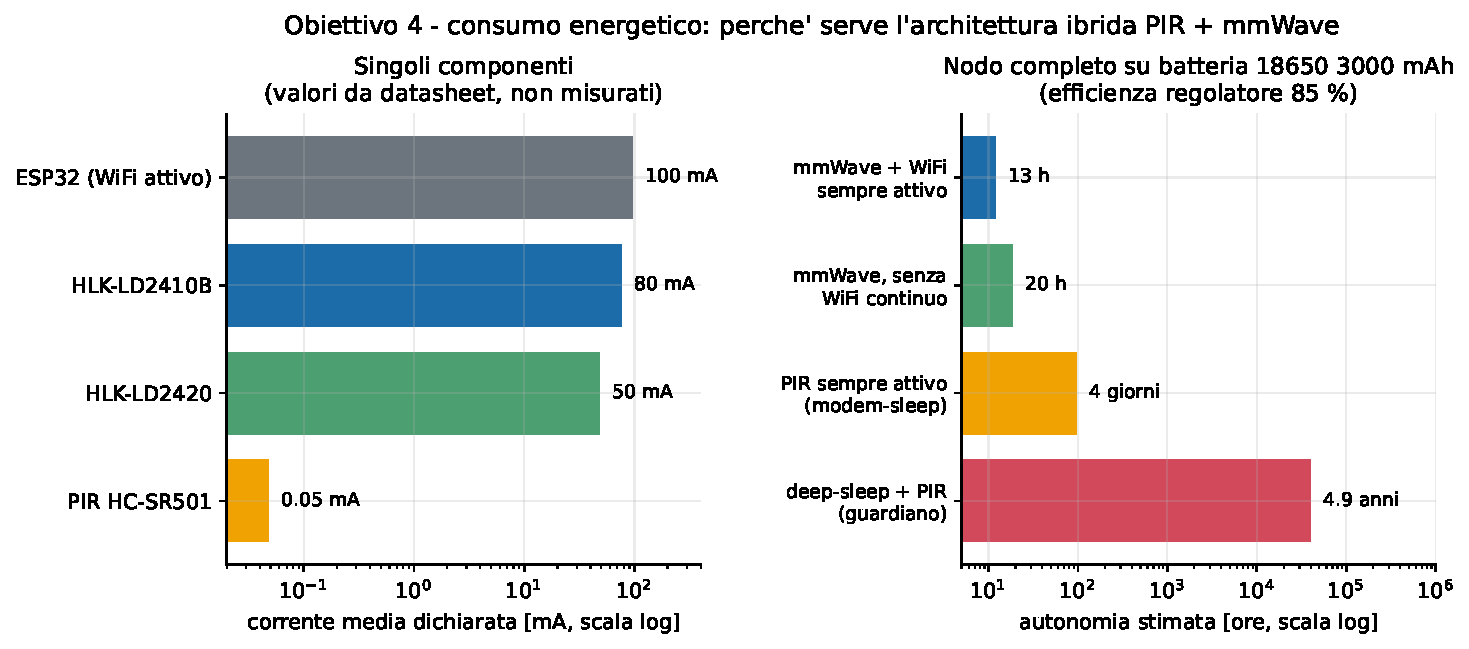
\includegraphics[width=\linewidth]{figures/fig13_consumi}
\caption{Consumi da datasheet dei singoli componenti e autonomia stimata dei nodi
completi, in scala logaritmica.}
\label{fig:consumi}
\end{figure}

\section{Implicazione per DIPME: l'architettura ibrida}
\label{sec:architettura-ibrida}

I numeri precedenti risolvono un'apparente contraddizione del progetto. Il nodo
integrato negli arredi deve restare in attesa per anni in tempo di pace e deve
funzionare a batteria durante il blackout che segue il sisma. I due requisiti sono
incompatibili con un sensore da 80~mA sempre acceso, ma anche con un sensore che non
vede le persone ferme (Capitolo~\ref{chap:confronto}). La soluzione non è scegliere fra i due
sensori ma metterli in sequenza temporale.

\begin{enumerate}[leftmargin=1.8em,itemsep=3pt]
  \item \textbf{Tempo di pace.} Il nodo resta in deep-sleep e si risveglia allo scadere del polling oppure quando il PIR rileva una presenza, come già fa il nodo del progetto~\cite{callisto2026dipme}. Il consumo è dell'ordine dei microampere e l'autonomia è pluriennale. Durante le lezioni però il PIR sveglia il nodo di continuo, quindi i 4,9 anni al solo consumo sono un limite superiore e l'autonomia reale dipende da quanto spesso l'aula è occupata.
  \item \textbf{Emergenza.} Al passaggio in emergenza, comandato come descritto nella Sezione~\ref{sec:dipme}, si accende il radar, che rileva anche la persona ferma sotto il banco e calcola l'indice di vitalità. L'autonomia di circa 20~ore (13 con il WiFi della web UI) copre la
        finestra critica iniziale delle operazioni di ricerca e soccorso.
  \item \textbf{Estensione della finestra.} Per coprire le prime 72~ore, l'orizzonte
        convenzionale del soccorso, si può maggiorare la batteria oppure alternare il
        radar con un ciclo di lavoro. Un minuto acceso ogni cinque, con l'ESP32 in light-sleep fra un'accensione e l'altra, riduce il consumo medio di circa cinque volte e porta l'autonomia oltre le 72~ore. Il prezzo è
        una latenza di rilevamento fino a quattro minuti, accettabile in questo
        scenario, perché la domanda è se c'è qualcuno sotto il banco e non in quale istante si è mosso. Resta da verificare che il radar, appena riacceso, rilevi subito una persona immobile già presente, perché sull'\ldb\ non è stato misurato e sull'\ldc\ un corpo vicino all'accensione altera la stima del fondo (Sezione~\ref{sec:ld2420-risultati}).
\end{enumerate}

Il PIR quindi non va sostituito. Non è un concorrente del radar ma il guardiano a
basso costo che decide quando accenderlo, mentre il radar resta lo strumento di misura
della fase di emergenza. I dati del Capitolo~\ref{chap:confronto} e quelli di questo
capitolo lo mostrano da due direzioni opposte. Anche fra gli sviluppi futuri della piattaforma compare la combinazione della presenza con gli altri segnali del nodo~\cite{callisto2026dipme}. Il Capitolo~\ref{chap:conclusioni} riprende questa architettura fra le
raccomandazioni per il progetto.
